\documentclass[12pt]{article}
\usepackage{array}
\usepackage{amsmath}
\usepackage{amssymb}
\usepackage{mathtools}
\usepackage{textcomp}
\usepackage{gensymb}
\usepackage{graphicx}
\usepackage{float}
\usepackage{caption}
\usepackage{amsfonts}
\usepackage[margin=1in]{geometry}

\newcounter{results}
\newcounter{questions}

\def\neg{{\sim}}
\def\Z{\mathbb{Z}}
\def\N{\mathbb{N}}
\def\R{\mathbb{R}}
\def\Q{\mathbb{Q}}
\def\E{\mathbb{E}}
\def\qed{\(\blacksquare\)}
\newcommand{\result}[1]{\stepcounter{results}{\bfseries Result \arabic{results}}: #1}
\newcommand{\question}[1]{\stepcounter{questions}{\bf \arabic{questions}}: #1}
\newenvironment{proof}[2][Proof]{\result{#2}\begin{trivlist} 
    \item[\hskip \labelsep {\sc #1:}]}{\qed\end{trivlist}}

\begin{document}
    \title{Computational Assignment \#2}
    \author{Ryan Coyne}
    \maketitle

    The multiplicity of two large interacting Einstein solids, with total energy \(q\), can be approximated by the equation \(\Omega = \left( \frac{e}{N} \right)^{2N}(q_Aq_B)^N\), where \(e\) is Euler's number, \(N\) is the number of oscillators in the solid, \(q_A\) is the total energy of solid A and \(q_B\) is the total energy of solid B. The energies of each solid are related by the equation \(q_A=q-q_B\). If we let \(z = q_A/q\), then, neglecting a constant portion, the multiplicity function is \(\left[ 4z(1-z) \right]^N\), which is plotted in Figure 1. The Gaussian function, \(\Omega = \Omega_{max}\cdot e^{-N(2x/q)^2}\), is plotted for \(\Omega_{max}=1\) in Figure 2. Both functions are initially plotted for \(N=1,10,100,1000,10000\). 
    
    \begin{figure}[h]
        \caption{Multiplicity Function}
        \centering
        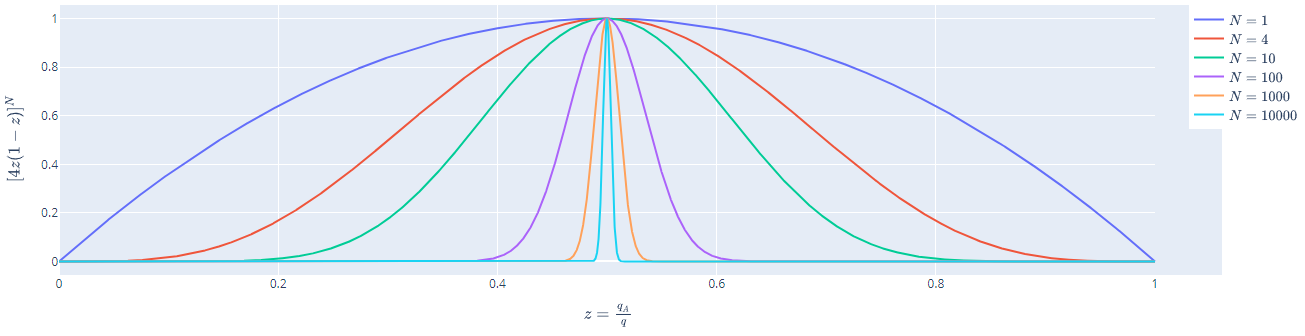
\includegraphics[width=\linewidth]{multiplicity.png}
    \end{figure}

    \begin{figure}[h]
        \caption{Gaussian Function}
        \centering
        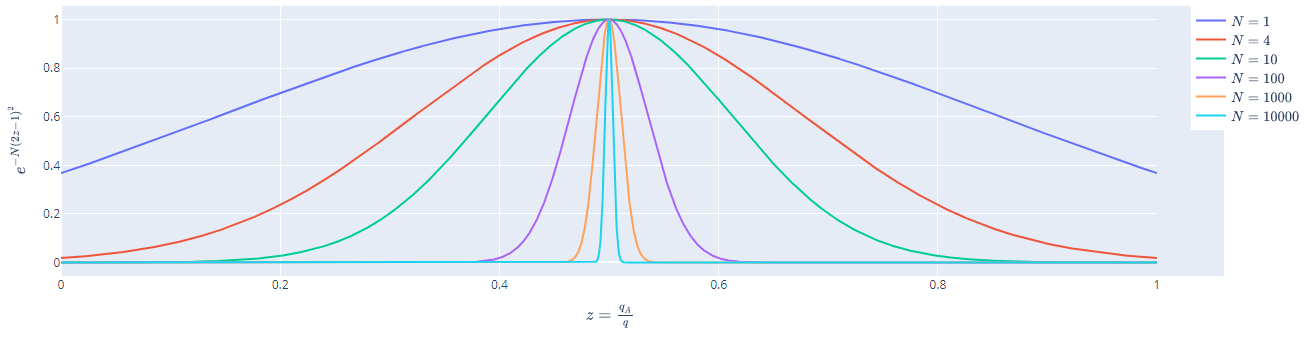
\includegraphics[width=\linewidth]{gaussian.png}
    \end{figure}
    
    If the difference in the full width at half maximum of the two plots is less than \(5\%\), then we say that the two distributions are the same. Of the given values of \(N\), the plots are the same for \(N=10, 100, 1000, 10000\). The smallest integer value of \(N\) for which they are the same is \(N=4\). The normalized distribution, or probability density function, is of the multiplicity is \(\frac{\Gamma(2+2N)}{4^N(\Gamma(N))^2} \left[ 4z(1-z) \right]^N\) and the probability density function for the gaussian is \(\frac{2\sqrt{N}}{\sqrt{\pi}\mathrm{erf}(\sqrt{N})} e^{-N(2x/q)^2}\).

\end{document}